
\chapter{Reproducibility}

\citet{chen2021relation} had studied the impact of relation prediction as an auxiliary training objective on the performance of KGE models. Their experimental study showed that, by incorporating relation prediction into entity ranking as a new training objective, the performance of models on Entity Ranking improved significantly \citep{chen2021relation}. However, the performance of relation prediction of the models was not studied, and the impact of relation prediction on model selection was not examined. Therefore, it is interesting to study the impact of relation prediction not only on entity ranking but also in relation to prediction performance, thus, to have fairness in the comparative study (Chapter \ref{cha:comparative_study}), it is essential to reproduce the models found by \citet{chen2021relation} using LibKGE \citep{libkge}. 
% and analyze the factors positively affecting to the performance of models. Finally, we determine the main factors that truly bring positive impact to performance of models.

By using LibKGE \cite{libkge} python-library for implementation, we can utilize its modular design which can give us flexibility when designing/running experiments \cite{Ruffinelli2020You}. Furthermore, LibKGE also provides the framework for KGE models, therefore, we can save time on re-implementation.

% We can easily see that factor is a main impact.

\section{Preliminary results}

In the paper, \citet{chen2021relation} conducted experiments on the ComplEx model with the nuclear 3-norm (N3) regularizer and Adagrad optimizer. There are three training types: entity prediction, and relation prediction, and both of them, i.e, entity and relation predictions. The model was trained for at most 400 epochs with a binary cross-entropy (BCE) loss function and 1vsAll \citep{Ruffinelli2020You}. Hyperparameter optimization was carried out using a grid search with 5 different hyperparameters: embedding size (\textit{d}), learning rate (\textit{lr}), batch size (\textit{bsz}) and weight of regularizer (\textit{reg}), and weight of relation prediction ($\lambda$). The first 4 hyper-parameters are shown in Table \ref{tab:AKBC grid search}. For WN18RR, the weight of relation prediction ($\lambda$) was searched over \{0.005, 0.001, 0.05, 0.1, 0.5, 1\}. For FB15k-237, \citet{chen2021relation} searched over \{0.125, 0.25, 0.5, 1, 2, 4\}. The best configuration for each of the datasets was chosen based on MRR.  Table \ref{tab:AKBC best models}shows the best configuration found by \citet{chen2021relation}.

\begin{table}[!htbp]
\centering
\caption{Grid Search \citep{chen2021relation}}
\label{tab:AKBC grid search}
\resizebox{\textwidth}{!}{%
\begin{tabular}{@{}lllll@{}}
\toprule
\textbf{Dataset} & \textit{d} \tablefootnote{The embedding size was written follow LibKGE}            & \textit{lr}     & \textit{bsz}         & \textit{reg}  \\ \midrule
FB15k-237        & \{200, 1000, 2000\} & \{0.1, 0.01\} & \{100, 500, 1000\} & \{0.0005, 0.005, 0.01, 0.05, 0.1, 0.5, 1, 0\} \\ 
WN18RR           & \{200, 1000, 2000\} & \{0.1, 0.01\} & \{100, 500, 1000\} & \{0.005, 0.01, 0.05, 0.1, 0.5, 1\}            \\ \bottomrule
\end{tabular}%
}
\end{table}


\begin{table}[!htbp]
\centering
\caption{The best ComplEx configurations found by \citet{chen2021relation}}
\label{tab:AKBC best models}
\resizebox{\textwidth}{!}{%
\begin{tabular}{@{}lllllllll@{}}
\toprule
Dataset   & Entity Prediction & Relation Prediction & \textit{d} & \textit{lr} & \textit{bsz}  & \textit{reg}    & $\lambda$  & MRR      \\ \midrule
FB15K-237 & Yes               & No                  & 2000       & 0.10        & 100  & 0.05   & NA         & 0.372305 \\
          & Yes               & Yes                 & 2000       & 0.10        & 1000 & 0.05   & 4.00       & 0.393722 \\
          & No                & Yes                 & 2000       & 0.10        & 1000 & 0.0005 & NA         & 0.262888 \\ \midrule
WN18RR    & Yes               & No                  & 2000       & 0.10        & 100  & 0.10   & NA         & 0.488083 \\
          & Yes               & Yes                 & 2000       & 0.10        & 100  & 0.10   & 0.05       & 0.490053 \\
          & No                & Yes                 & 2000       & 0.10        & 500  & 0.5    & NA         & 0.257945 \\ \bottomrule
\end{tabular}%
}
\end{table}


The nuclear 3-norm regularizer was written by \citet{lacroix2018canonical} as $\| u_r^{(d)} \|^3_p = \sum_{j=1}^{n_d}|u_{r,j}^{(d)}|^3$. The N3 is implemented by using this formulation of the form:  
\begin{equation}
\label{eq:minization function}
\min_{(u_r^{(d)})_{\substack{d=1\dots3 \\ r=1\dots R}}}\displaystyle\sum_{(i,j,k)\in \mathit{S}}[l_{i,j,k}(\displaystyle\sum_{r=1}^R u_r^{(1)} \otimes u_r^{(2)} \otimes u_r^{(3)}) + \frac{\mathrm{w}}{3}\displaystyle\sum_{r=1}^R (|u_{r,i}^{(1)}|^3 + |u_{r,j}^{(2)}|^3 + |u_{r,k}^{(3)}|^3)]
\end{equation}

The N3 was implemented in LibKGE as L3 regularizer \citep{Ruffinelli2020You}.

\subsection{Similarly setting}
To obtain the best ComplEx models reported by \citet{chen2021relation}, we set the hyperparameters for ComplEx models using the best configurations founded by \citet{chen2021relation} and trained them using LibKGE (for more details, see Appendix \ref{cha:appendix-AKBC preproducibility}). Besides that, to ensure that we have the same models like them, the performance of models obtained from LibKGE were checked against the performance of models obtained by using their codebase \footnote{\citet{chen2021relation}'s code base Github: https://github.com/facebookresearch/ssl-relation-prediction}. Cross-checking was performed by comparing model performance on the "validation dataset" in three key metrics: MRR, Hits@1, Hits@3, and Hits@10. The cross-checking results was shown in Table\ref{tab:best config from AKBC}.

As can be seen, there were huge differences between models from the \citet{chen2021relation} code base and models produced from LibKGE. For example, the performance models trained with entity and relation prediction from LibKGE are lower than from \citet{chen2021relation}, (i.e., 0.362 in MRR and 0.388 in MRR respectively). Furthermore, with the same hyper-parameter configurations, the model trained on relation prediction only from LibKGE performed much better than the model from \citet{chen2021relation} on WN18RR (i.e. 0.430 in MRR and 0.258 in MRR respectively). It indicated that there should be differences in the implementation between the two codebases. Thus, it is necessary to perform an open hyperparameter optimization with previous knowledge about the implementation from \citet{chen2021relation}.

\begin{table}[!htbp]
\centering
\caption{Reproduction results of the best models of \citet{chen2021relation} using LibKGE}
\label{tab:best config from AKBC}
\resizebox{\textwidth}{!}{%
\begin{tabular}{lllllllllll}
\hline
Dataset   & Entity Prediction & Relation Prediction & \multicolumn{4}{c}{\parbox[t]{5cm}{\centering Entity Ranking from \citet{chen2021relation}'s code base} \vspace{0.1cm}} & \multicolumn{4}{c}{Entity Ranking from LibKGE} \\
          &                   &                     & MRR    & Hits@1 & Hits@3 & Hits@10 & MRR       & Hits@1    & Hits@3    & Hits@10    \\ \hline
FB15K-237 & Yes               & No                  & 0.366  & 0.271  & 0.401  & 0.557   & 0.357     & 0.266     & 0.392     & 0.540      \\
          & Yes               & Yes                 & 0.388  & 0.298  & 0.425  & 0.568   & 0.362     & 0.272     & 0.397     & 0.546      \\
          & No                & Yes                 & 0.263  & 0.187  & 0.287  & 0.411   & 0.261     & 0.187     & 0.283     & 0.408      \\ \hline
WN18RR    & Yes               & No                  & 0.487  & 0.441  & 0.501  & 0.58    & 0.475     & 0.438     & 0.489     & 0.552      \\
          & Yes               & Yes                 & 0.488  & 0.443  & 0.505  & 0.578   & 0.475     & 0.437     & 0.490     & 0.550      \\
          & No                & Yes                 & 0.258  & 0.212  & 0.29   & 0.339   & 0.430     & 0.384     & 0.454     & 0.511      \\ \hline
\end{tabular}%
}
\end{table}

\subsection{Random Hyper-parameter search}
The hyper-parameter searching space was conducted using a random search with the same five hyper-parameters (Table \ref{tab:open-search}).


\begin{table}[!htbp]
\centering
\caption{Open hyper-parameter search to find \cite{chen2021relation}'s best models}
\label{tab:open-search}
\resizebox{\textwidth}{!}{%
\begin{tabular}{@{}lllll@{}}
\toprule
\multicolumn{1}{c}{\multirow{2}{*}{Dataset}} & \multicolumn{2}{c}{WN18RR}                                & \multicolumn{2}{c}{FB15k-237}                                       \\
\multicolumn{1}{c}{}                         & \citet{chen2021relation}            & LibKGE              & \citet{chen2021relation}                      & LibKGE              \\ \midrule
\textit{d}                                   & \{200, 1000, 2000\}                 & \{200, 1000, 2000\} & \{200, 1000, 2000\}                           & \{200, 1000, 2000\} \\
\textit{lr}                                  & \{0.1, 0.01\}                       & {[}0.01, 0.1{]}     & \{0.1, 0.01\}                                 & {[}0.01, 0.1{]}     \\
\textit{bsz}                                 & \{100, 500, 1000\}                  & \{100, 500, 1000\}  & \{100, 500, 1000\}                            & \{100, 500, 1000\}  \\
\textit{reg}                                 & \{0.005, 0.01, 0.05, 0.1, 0.5, 1\}  & {[}0.001, 1{]}      & \{0.0005, 0.005, 0.01, 0.05, 0.1, 0.5, 1, 0\} & {[}0.0005, 1{]}      \\
$\lambda$                                    & \{0.005, 0.001, 0.05, 0.1, 0.5, 1\} & {[}0.005, 1{]}      & \{0.125, 0.25, 0.5, 1, 2, 4\}                 & {[}0.125, 4{]}        \\ \bottomrule
\end{tabular}%
}
\end{table}

\section{The differences in the two codebases}

There are two main differences between the two code bases; instead of training ComplEx directly on the original dataset, the models were trained with reciprocal triples included in the dataset \citep{chen2021relation}. Furthermore, there is a difference in regularization implementation.


\subsection{Reciprocal relations}

\noindent\textbf{Including reciprocal triplets}
The reciprocal relations technique was introduced by \citet{kazemi2018simple} and \citet{lacroix2018canonical} to decrease computational cost, and it may lead to better performance \citep{lacroix2018canonical}. The key idea is that instead of using the same scoring function to predict object \textit{(s,p,?)} and subject \textit{(?,p,o)}, the prediction is made by two separate scoring functions, one for the prediction of objects and one for the prediction of subjects. To achieve that, both scoring functions share the same entity embeddings; however, they do not share the same relation embedding (i.e., each relation contains two embeddings).

In order to apply the reciprocal relation technique, \citet{chen2021relation} intentionally modified the training dataset as follows (for details of implementation, see Appendix \ref{sec:AKBC Reciprocal dataset}): (1) the original dataset is duplicated, (2) those object entities of the duplicated dataset was swapped for the subject entities, finally (3), the relation ids of those triplets are shifted to new ids by adding the number of relations. Therefore, the number of subject and object entities examined in one epoch is double than a dataset without reciprocal triplets. Due to duplication, their models are trained only on object prediction, that is, answering \textit{(s,p,?)}

While, in LibKGE, preserving the training dataset is mandatory, thus, to apply the reciprocal relation technique, the total number of relation embeddings need to be doubled compared to original number of relation in dataset. Furthermore, the models need to be trained with entity prediction, that is, including object prediction \textit{(s,p,?)} and subject prediction \textit{(?,p,o)} at the same time. 


Based on these observations, it implies that entities (subjects and objects) in their code base are regularized twice as much as in LibKGE. Therefore, for example, instead of 0.05, 0.0005, 0.1 and 0.5 as shown in Table \ref{tab:AKBC best models}, the weight of regularization for entity embeddings should be 0.1, 0.001, 0.2 and 1 respectively.
\newline

\noindent\textbf{Relation prediction in reciprocal relational model}
When applying the reciprocal relation technique, we introduce two different embeddings for a single relation: the original relation and reciprocal relation embedding. Therefore, to perform the relation prediction \textit{(s,?,o)}, it is still an open question whether the models should consider all the embeddings of the relations or just consider all the original relations and reciprocal relations separately. In their code base, \citet{chen2021relation} decided to use all of the relation predictions instead of considering part of them.  

\subsection{Regularization implementation}


\noindent\textbf{The nuclear 3-norm.} Instead of scaling them one-third as in Equation \ref{eq:n3}, \citet{chen2021relation} omitted them and decided to use only the sum. While in LibKGE, the formula is preserved as it is; thus, it implies that entities and relation embeddings in their code base are regularized thrice as much as in LibKGE.

Based on these observations from the reciprocal relation and the N3 implementation, the regularization weight of entity embedding and relation embeddings should be 6 times for entity and 3 times for relation. The table \ref{tab:Reg for emb} shows the equivalence between those two code bases.
\newline

% Please add the following required packages to your document preamble:
% \usepackage{graphicx}
\begin{table}[!htbp]
\centering
\caption{Equivalence of regularization weights in two codebases}
\label{tab:Reg for emb}
\resizebox{\textwidth}{!}{%
\begin{tabular}{lllcccc}
\hline
Dataset   & Entity Prediction & Relation Prediction & \multicolumn{2}{c}{\citet{chen2021relation}}                                      & \multicolumn{2}{c}{LibKGE}                                \\
          &                   &                     & \multicolumn{1}{l}{Entity} & \multicolumn{1}{l}{Relation} & \multicolumn{1}{l}{Entity} & \multicolumn{1}{l}{Relation} \\ \hline
FB15K-237 & Yes               & No                  & 0.05                       & 0.05                         & 0.3                        & 0.15                         \\
          & Yes               & Yes                 & 0.05                       & 0.05                         & 0.3                        & 0.15                         \\
          & No                & Yes                 & 0.0005                     & 0.0005                       & 0.003                      & 0.0015                       \\ \hline
WN18RR    & Yes               & No                  & 0.1                        & 0.1                          & 0.6                        & 0.3                          \\
          & Yes               & Yes                 & 0.1                        & 0.1                          & 0.6                        & 0.3                          \\
          & No                & Yes                 & 0.5                        & 0.5                          & 3.0                        & 1.5                          \\ \hline
\end{tabular}%
}
\end{table}


\noindent\textbf{Regularizing Complex embedding vectors.} In LibKGE, we regularize the entities and relations directly on embedding vectors \citep{Ruffinelli2020You}. However, in \citet{chen2021relation} and \citet{lacroix2018canonical} codebases, the entity and relation embeddings of ComplEx model are normalized by L2-norm before being regularized by the L2 or N3 regularization. 

L3 or N3 regularization of a embedding vector $u$ is a norm of a vector which is defined as:
\begin{equation}
    \label{eq:N3}
    \|u \|^3_p = \sum_{j=1}^{n_d}|u_j|^3
\end{equation} 

For the ComplEx model, a embedding vector is a complex vector $u \in \mathbb{C}^K$ which is composed of a real vector component and an imaginary vector component. Let denote $u_j = u'_j + iu''_j$. Therefore the norm of a complex number is defined as $|u_j| = \sqrt{{u'}_j^2 + {u''}_j^2}$. Put it into Formula \ref{eq:N3}, we have:
\begin{equation}
    \label{eq:final}
    \|u \|^3_p = \sum_{j=1}^{n_d}|u_j|^3 = \sum_{j=1}^{n_d}\left(\sqrt{{u'}_j^2 + {u''}_j^2}\right)^3
\end{equation} 


More precisely, a embedding vector in ComplEx model is a complex vector $u \in \mathbb{C}^K$ which is composed of a real vector component and an imaginary vector component. 

Each of  formed by two part: real part and imaginary part \citet{trouillon2016complex}. Technically, 

each of complex component in embedding vector will be normalized based on 
\newline

\subsection{Ablation study}


\begin{figure}[!htbp]
	\begin{center}
	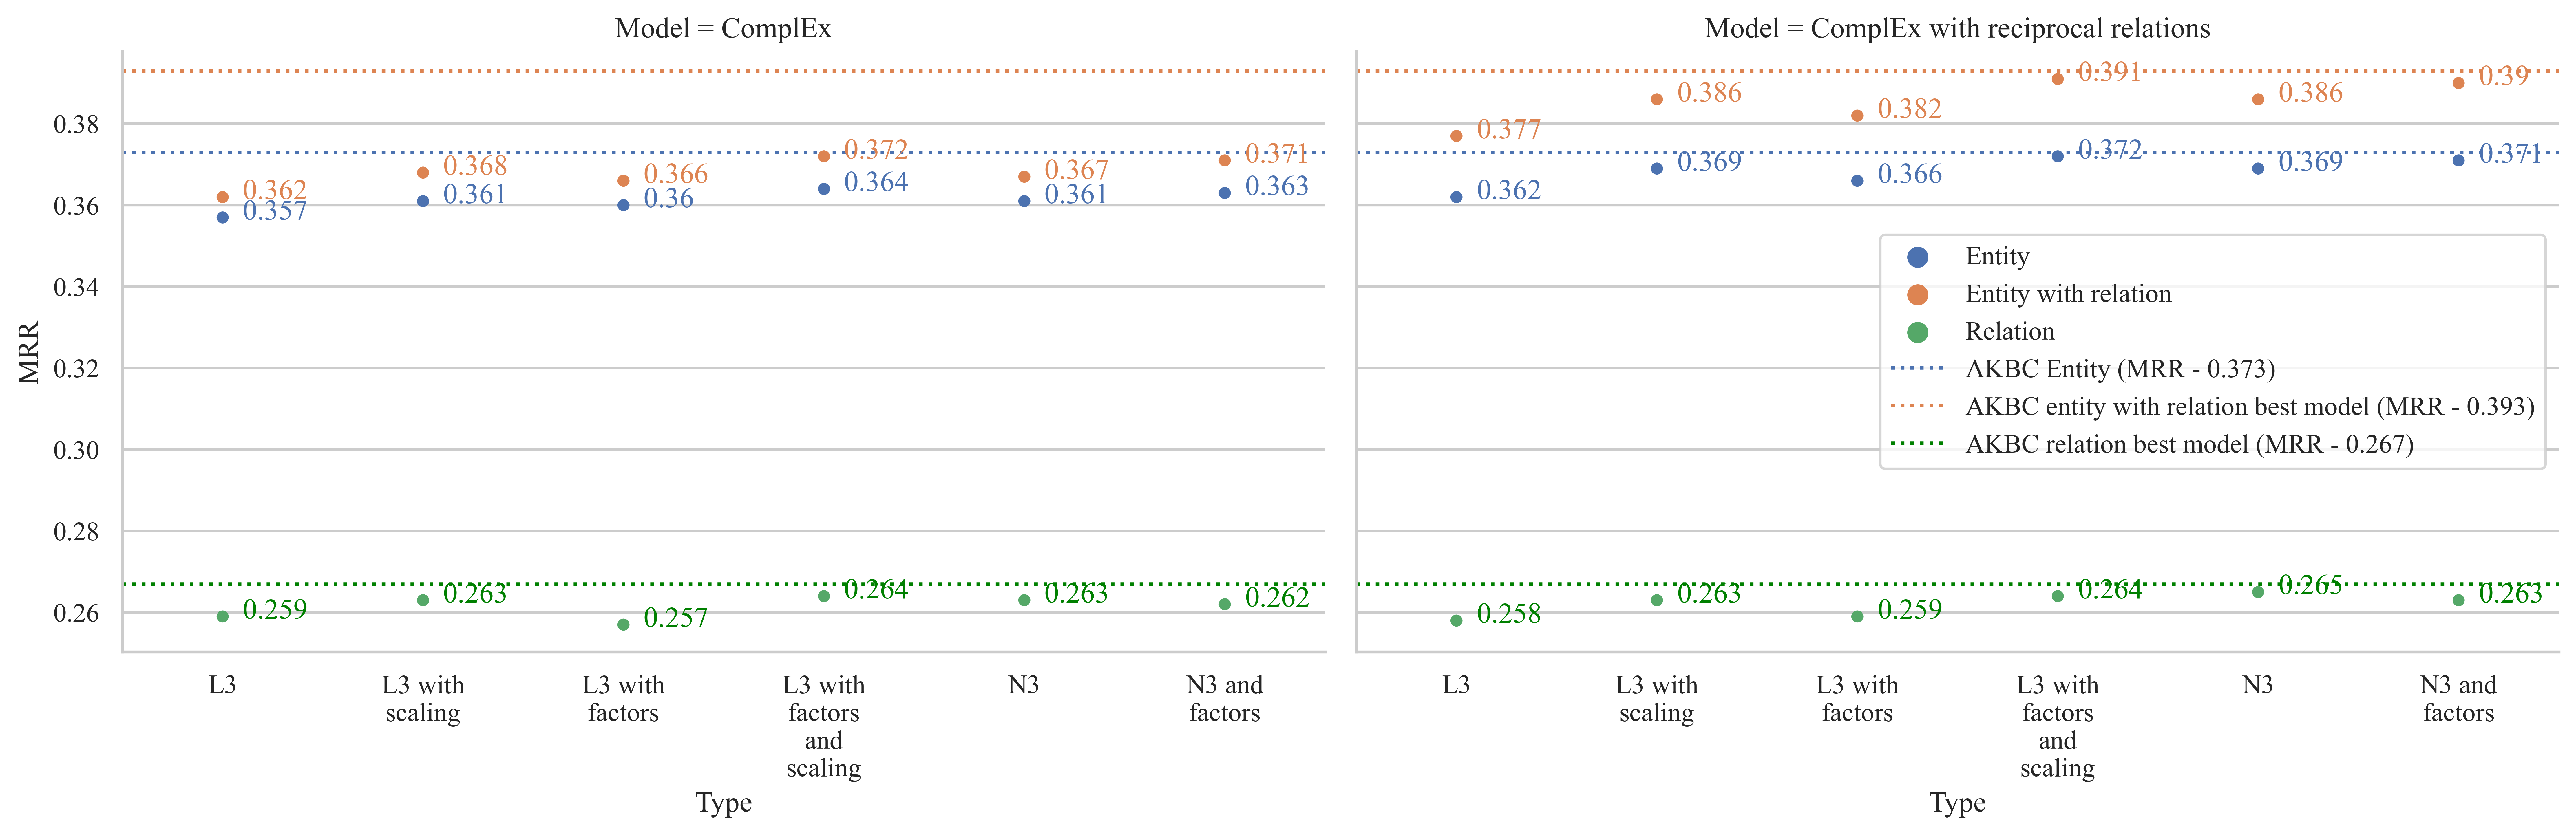
\includegraphics[width=\linewidth]{Images/Ablation_FB237.png}
	\caption[Ablation FB237]{Ablation FB237}
	\label{fig:Ablation FB237}
	\end{center}
\end{figure}

\begin{figure}[!htbp]
	\begin{center}
	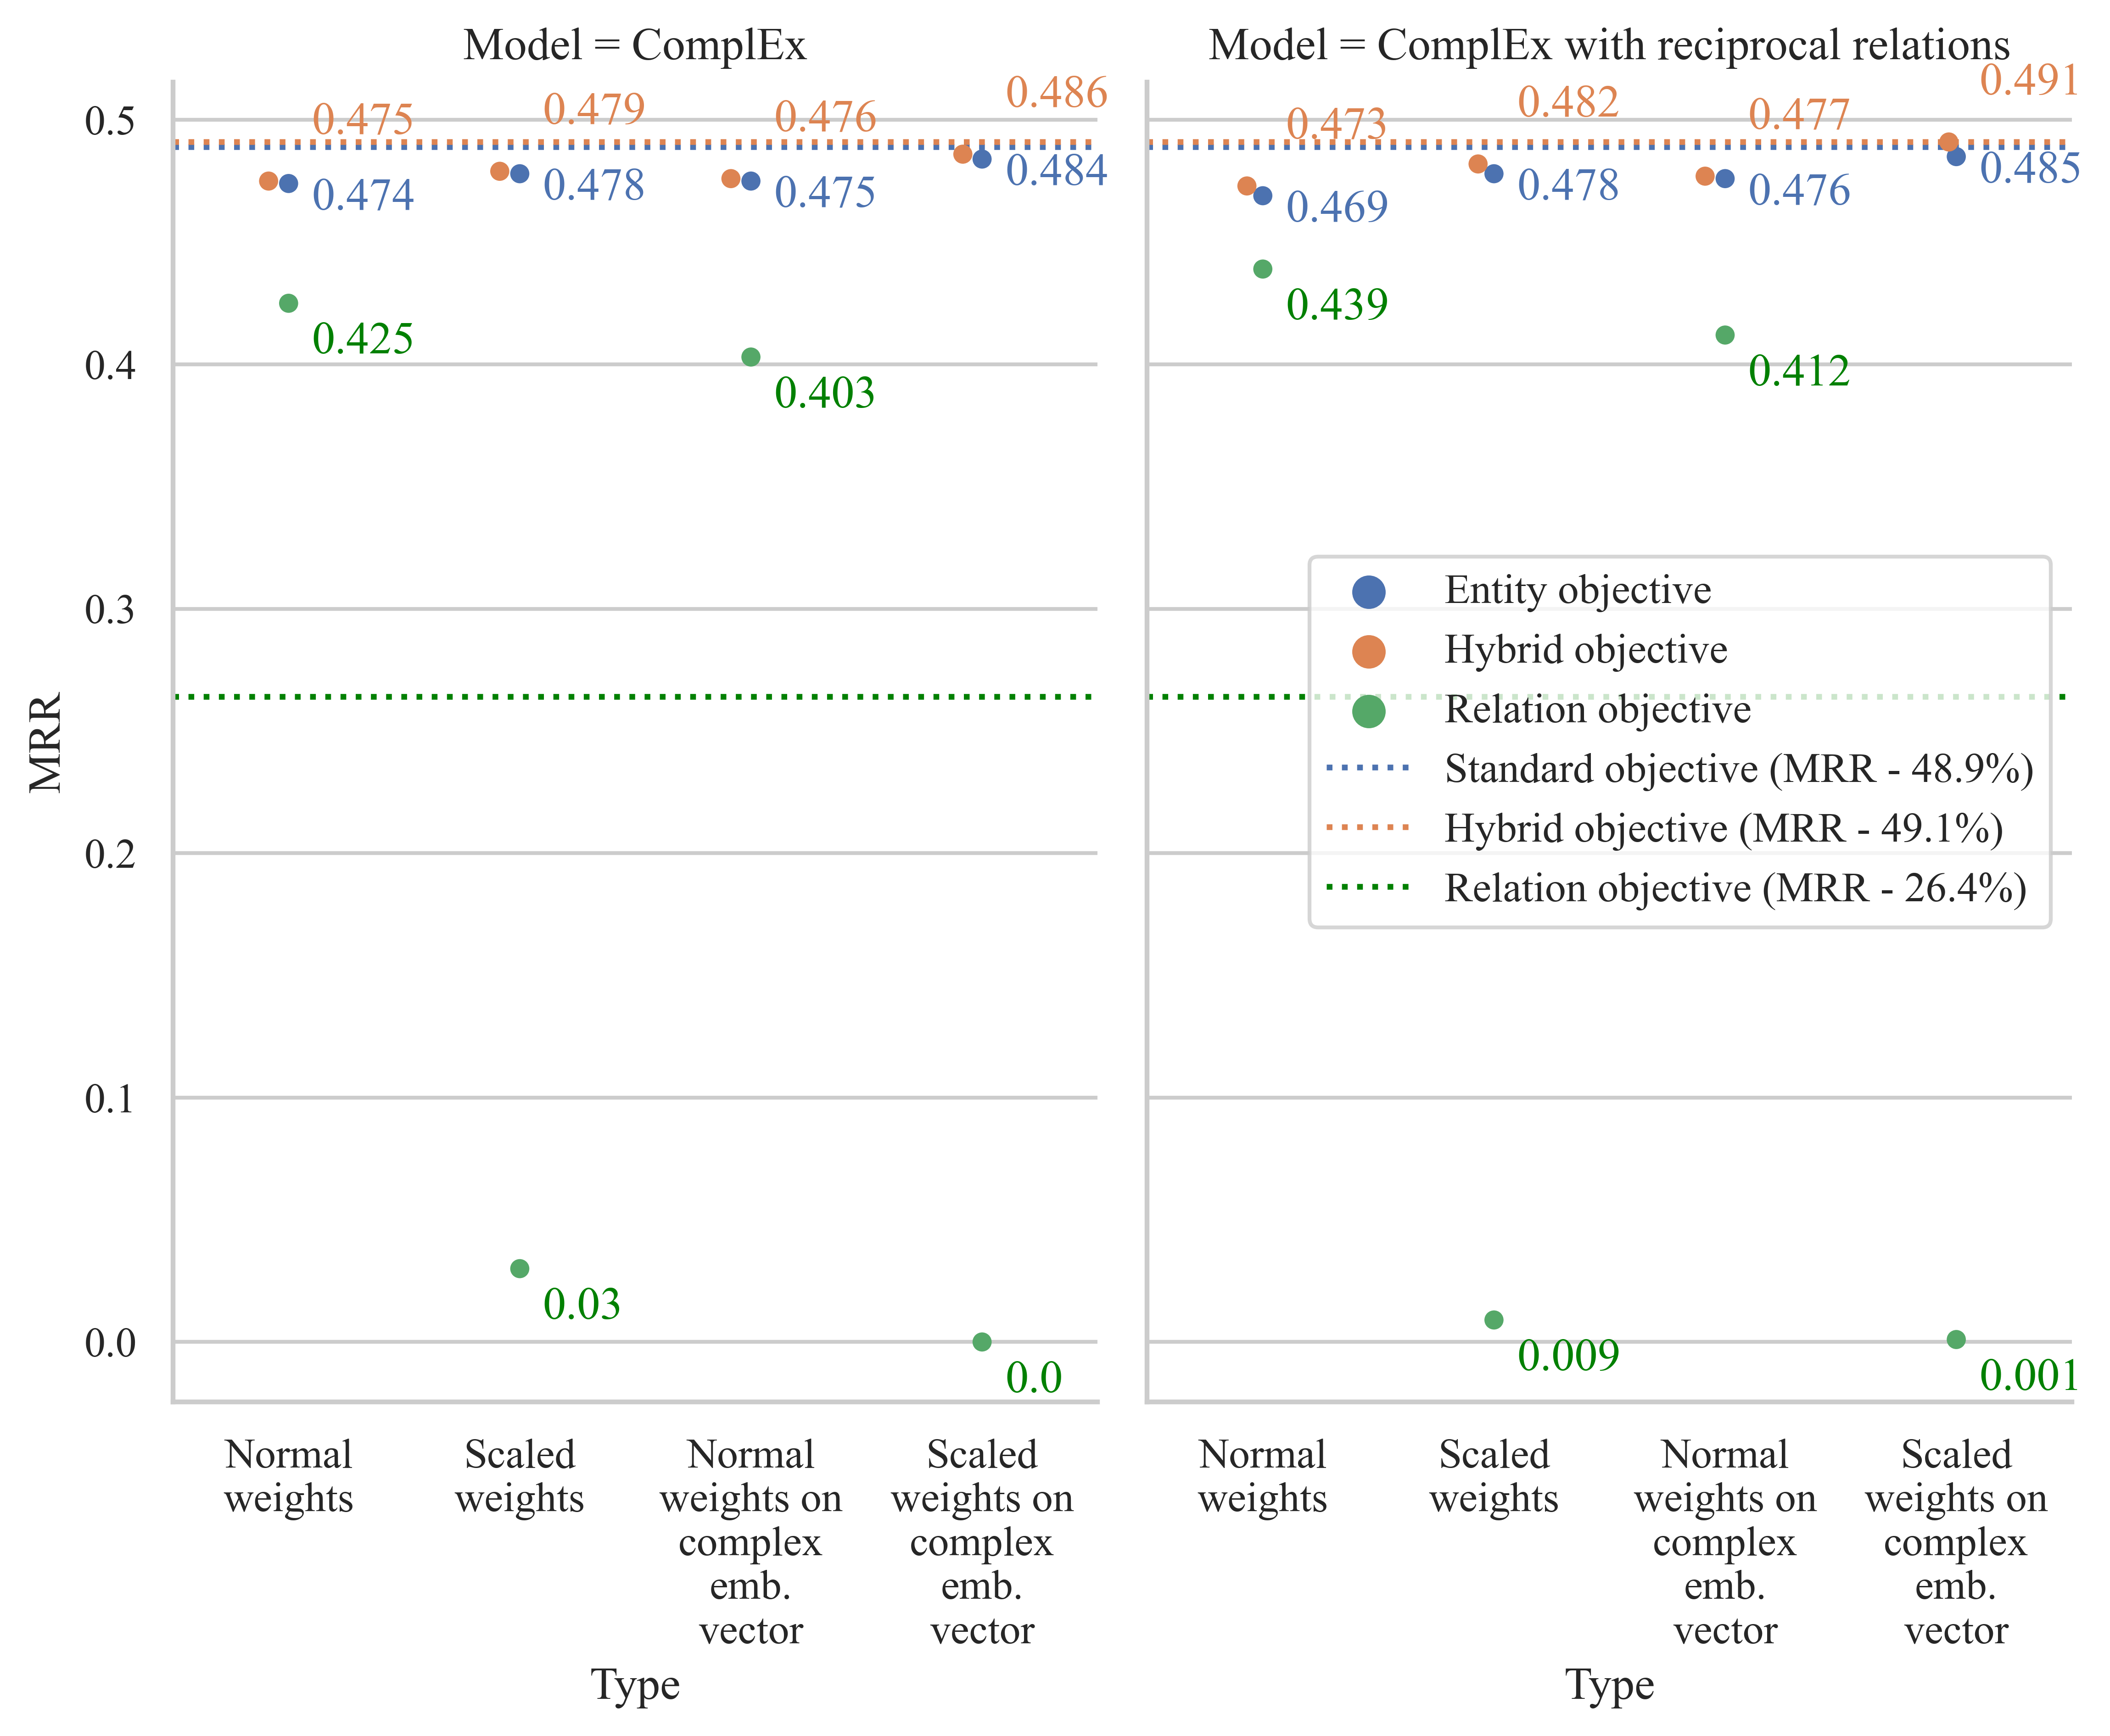
\includegraphics[width=\linewidth]{Images/Ablation_WNRR.png}
	\caption[Ablation WNRR]{Ablation WNRR}
	\label{fig:Ablation WNRR}
	\end{center}
\end{figure}